\documentclass[12pt,a4paper]{article}
\usepackage[utf8]{inputenc}
\usepackage[czech]{babel}
\usepackage{datetime}
\usepackage{tabularx}
\usepackage{graphicx}
\usepackage{float}
\renewcommand{\dateseparator}{. }
\begin{document}

\title{Řešení problému vážené splnitelnosti booleovské formule pokročilou iterativní metodou}
\author{Dominik Plíšek}
\date{\dmyyyydate\today}
\maketitle

\tableofcontents


\section{Úvod}

Zadáním je použít pokročilou iterativní metodu pro řešení problému splnitelnosti booleovské formule. Optimalizovanou hodnotou je celková váha tvořená součtem vah všech proměnných, které jsou ohodnoceny na TRUE. V této práci se budu zabývat metodou simulovaného ochlazování. 

Úlohu jsem se rozhodl omezit na klauzule velikosti tří proměnných, takzvaný problém 3SAT. Tato úloha není lehčí, ale snadněji se mi implementovala.

Vývoj řešičky budu provázet experimenty, které jsou prováděny na jednom vlákně procesoru 2,3 GHz Intel Core i7 s 6 MB L3 cache. Operační systém je Apple OS X verze 10.11.3.

Program je napsaný v C++ a staví na mé předchozí zkušenosti s metodou simulovaného ochlazování implementovanou za účelem řešení problému batohu. Práce na toto téma je k dispozici zde:

https://edux.fit.cvut.cz/courses/MI-PAA/student/plisedom/start\#uloha\_4.

Pro měření času jsem použil funci clock() z time.h, která vrací procesorový čas, čili měřil jsem, jak dlouho procesor na úloze skutečně pracoval, bez ohledu na režii operačního systému okolo.



\section{Implementační postupy}

\subsection{Struktura}
\label{structure}

Program je psaný v C++ a používá (do jisté míry) objektově orientované principy. Tři základní třídy jsou:

\begin{description}
    \item[SATInstance] Udržuje informace o instanci, umí načíst cnf formát a umí sama sebe randomizovat a řešit.
    \item[SATEvaluation] Obsahuje vektor ohodnocení proměnných instance, vektor splněných klauzulí, udržuje aktuální součet vah kladně ohodnocených proměnných a počet splněných formulí.
    \item[SATClause] Obsahuje svůj index, vektor proměnných a vektor jejich kladnosti
\end{description}

SATInstance obsahuje vektor všech klauzulí instance. V případě, kdy změníme nějaké ohodnocení proměnné, museli bychom celý tento vektor vždy projít, abychom našli, v kterých klauzulích je proměnná použita. Řešení jsem zvolil takové, že SATInstance obsahuje navíc vektor říkající, v kterých klauzulích je která proměnná obsažena. Ten je podstatně menší a přes něj se při změně hodnoty proměnné můžeme velice efektivně dostat ke všem klauzulím, jejichž celkové ohodnocení je třeba upravit.

\subsection{Postup řešení}

\subsubsection{Randomizace}

Nejprve je třeba zvolit počáteční ohodnocení. Toto volíme zcela náhodně. Nejprve projdeme všechny proměnné a náhodně je označíme jako TRUE/FALSE. Zároveň si připravujeme informaci o aktuální váze. Dále projdeme všechny klauzule instance a zapíšeme si, které klauzule jsou celkově ohodnoceny na TRUE a uložíme si tuto informaci spolu s informací o celkovém počtu kladně ohodnocených klauzulí.

\subsubsection{Ekvilibrium}

V průběhu řešení problému metodou simulovaného ochlazování je třeba v jistých intervalech snižovat teplotu. Rozhodnutí, zda dojde ke snížení teploty, se nazývá ekvilibrium. Zvolil jsem takovou podmínku, která sníží teplotu, máme-li již přijato tolik změn stavu, jaká je velikost instance (počet proměnných). 

Taková varianta by však narazila v případě, že je řešení přijímáno málo. Proto jsem implementoval ještě jednu podmínku, která říká, že teplotu je třeba snížit i tehdy, když zvážíme tolik změn stavů, kolik je dvojnásobek počtu proměnných.

\subsubsection{Hledání souseda}

Hledání souseda jsem se rozhodl provést tak, že vyberu náhodnou proměnnou a otočím její ohodnocení, tedy byla-li TRUE, je nyní FALSE, a naopak. Poté projdu všechny klauzule, které tuto proměnnou obsahují (seznam takových klauzulí mám předem připravený, viz sekce \ref{structure}).

\subsubsection{Přijetí horšího výsledku}

Ochota přijmout horší výsledek, než je aktuální, určena dána aktuální teplotou, která je postupně snižována, a to vzorcem:

\begin{verbatim}
    randFloat < exp(-diff / temp)
\end{verbatim}

kde randFloat je náhodné reálné číslo mezi 0 a 1, diff je rozdíl hodnoty předchozího a aktuálního ohodnocení (kladné diff znamená zhoršení) a temp je momentální teplota.


\subsubsection{Údržba dosud nejlepšího řešení}

Pokaždé, když najdeme ohodnocení, které má všechny klauzule kladné, uložíme jej jako nejlepší, pokud nemá horší váhu než ohodnocení, které již máme uloženo jako nejlepší. Na počátku je nejlepší řešení takové, které má váhu 0.



\subsubsection{Restart}

Nepodaří-li se nám nalézt touto metodou žádné ohodnocení, které má všechny klauzule kladné, dříve než metoda zmrzne, proběhne restart. To znamená, že zvýšíme globální informaci o počtu restartů a spouštíme metodu od začátku. Celkový počet kroků řešení i měřič času je globální, to znamená, že obaluje celý postup včetně restartů. 






\section{Volba parametrů}

\subsection{Počáteční teplota}

Jedním z rozhodnutí, které je třeba učinit, je způsob získání počáteční teploty. Tu lze volit fixně. Pak se ale může stát, že ji zvolíme příliš vysokou a metoda bude neefektivní, protože se bude dlouho potácet, aniž by konvergovala k nějakému minimu. To je vidět na obrázku \ref{tooHighStart}. Případně ji můžeme zvolit příliš nízkou, přičemž pak nastane situace, kdy metoda rychle uvízne v lokálním minimu a většinou ani nenalezne platný výsledek, proto se hned restartuje, viz obrázek \ref{tooLowStart}. Oba tyto grafy představují reálné běhy metody nad instancí CBS\_k3\_n100\_m403\_b30\_0.cnf při koeficientu ochlazování 0.99 a dynamicky odvozenou spodní hranicí teploty.

\begin{figure}[H]
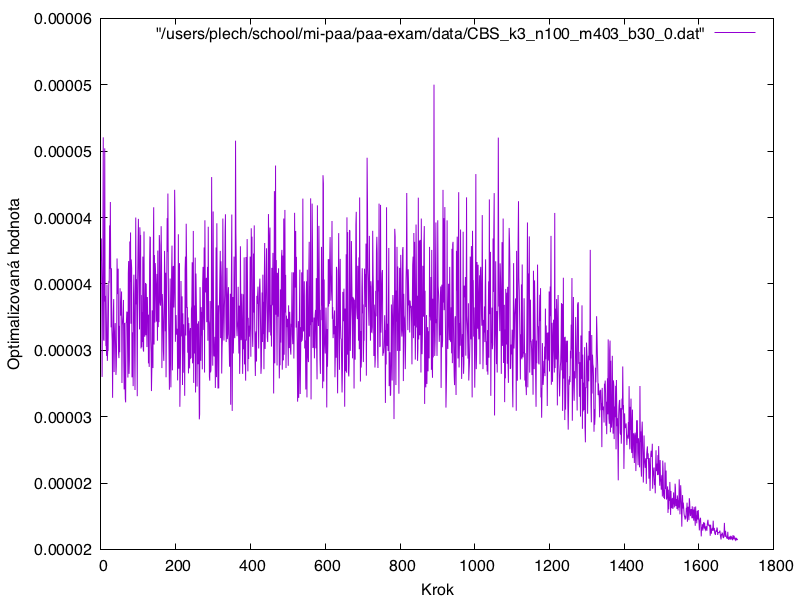
\includegraphics[width=\textwidth]{tooHighStart}
\caption{Příliš vysoká počáteční teplota}
\label{tooHighStart}
\end{figure}

\begin{figure}[H]
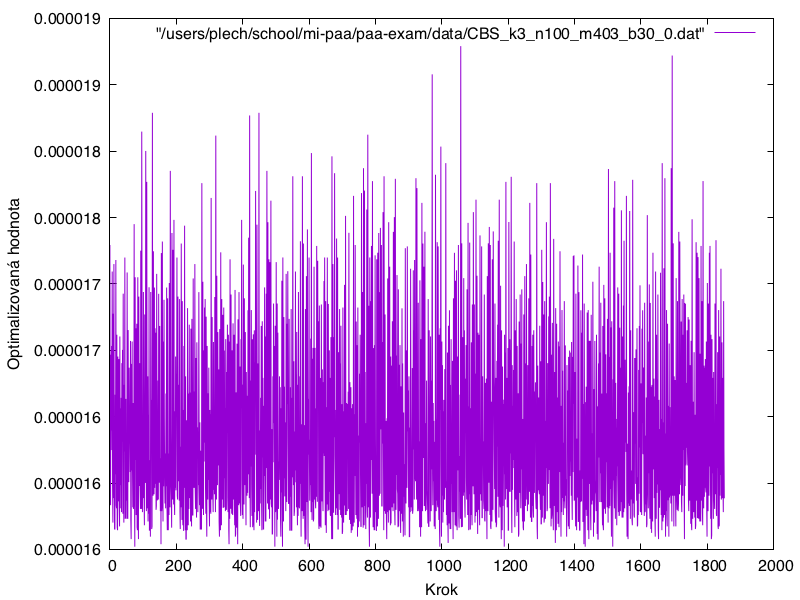
\includegraphics[width=\textwidth]{tooLowStart}
\caption{Příliš nízká počáteční teplota}
\label{tooLowStart}
\end{figure}

Dalším rozhodnutím je spodní mez teploty, tedy ta teplota, na níž se metoda zastaví. Tato opět lze volit fixně, ale může nastat problém, když zvolíme spodní hranici příliš vysoko. Metoda pak skončí dříve, než se dostane do fáze intensifikace, a většinou ani nenalezne platný výsledek, proto se hned restartuje, jak je vidět na obrázku \ref{tooHighEnd}. Při příliš nízké koncové teplotě můžeme zbytečně dlouho čekat na výsledek, který se již nemění, viz obrázek \ref{tooLowEnd}. Na tomto grafu jsou krásně vidět tři restarty, kde každý průbeh velice rychle klesl do minima a tam zůstal zbytečně dlouho. Oba tyto grafy představují reálné běhy metody nad instancí CBS\_k3\_n100\_m403\_b30\_0.cnf při koeficientu ochlazování 0.99 a dynamicky odvozenou horní hranicí teploty.

\begin{figure}[H]
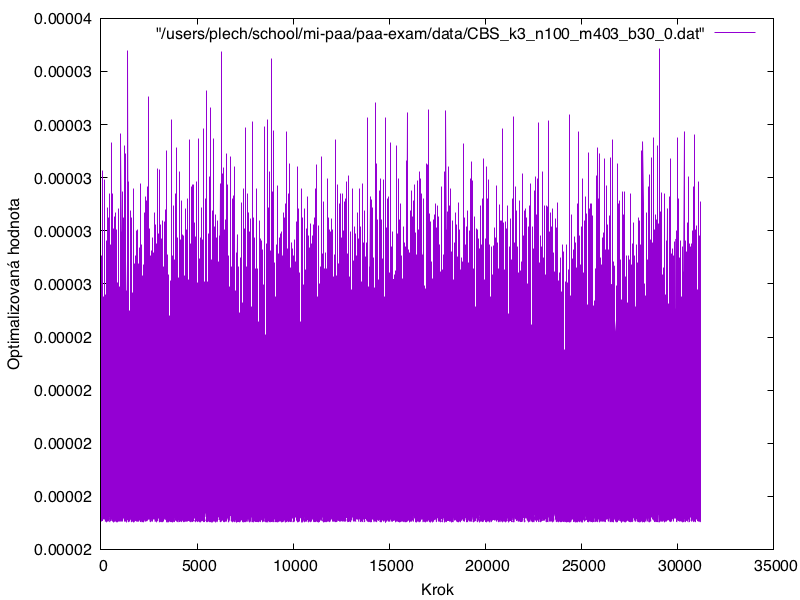
\includegraphics[width=\textwidth]{tooHighEnd}
\caption{Příliš vysoká koncová teplota}
\label{tooHighEnd}
\end{figure}

\begin{figure}[H]
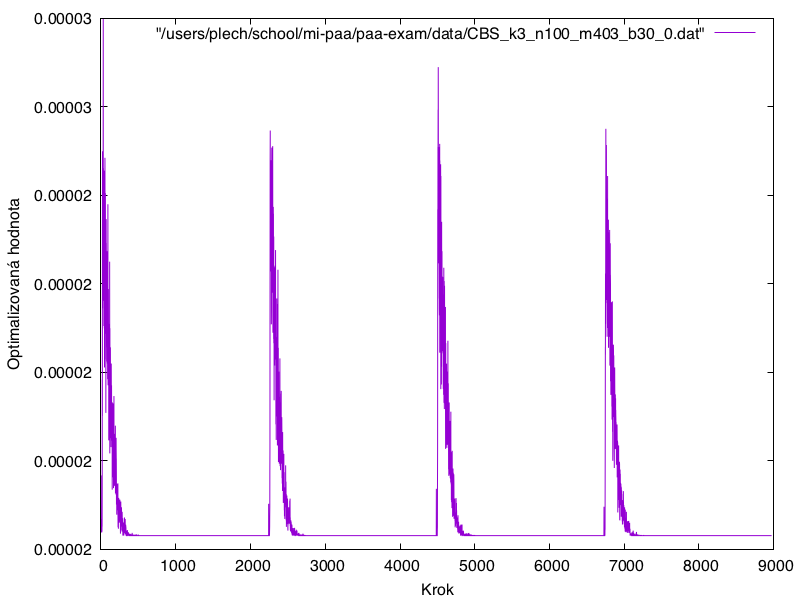
\includegraphics[width=\textwidth]{tooLowEnd}
\caption{Příliš nízká koncová teplota}
\label{tooLowEnd}
\end{figure}



Počáteční teplota lze spočítat. Místo abychom ji hádali, spustíme nejdříve ,,metodu prudkého ohřívání``. Ta začne na velmi nízké počáteční teplotě a rychle ji zvyšuje. Jakmile je dosaženo teploty, kdy je poloviční pravděpodobnost, že je přijat jako další stav stav horší, zaznamenáme tuto teplotu jako počáteční, a teprve potom spouštíme normální běh metody.

Tento postup jsem se rozhodl implementovat. Za rychlost ohřívání jsem zvolil parametr 1.5. Pro každou teplotu se spočítá počet přijatých skoků do sousedního stavu a kolik z nich jsou skoky k horšímu. Jakmile tento poměr dosáhne poloviny, zastaví se příprava, zaznamená se teplota a hlavní průběh metody se spustí s touto počáteční teplotou.


\subsection{Zmrznutí}

Koncová teplota lze též volit dynamicky. Lze počítat, kolik skoků se algoritmus rozhodl provést ze všech nabízených. V mém případě metoda tento poměr spočítá pro každou testovanou teplotu a dosáhne-li méně než 5\%, dojde ke ,,zmrznutí`` a metoda končí.







\subsection{Optimalizovaná hodnota}

Tato metoda naráží na zásadní problém, že v mnoha případech drtivá většina stavů (ohodnocení) není platným řešením, protože nemá všechny klauzule ohodnoceny na TRUE. Na rozdíl od problému batohu, který jsem touto metodou v minulosti řešil, nelze takové stavy prostě ignorovat, protože jich je velmi mnoho a postup by se snadno zcela zastavil. Bylo tedy třeba nasadit určité penále pro případ, že pracujeme se stavem, který není řešením.

Vzhledem k tomu, že metoda počítá s optimalizací ve smyslu minimalizace, pracoval jsem s výchozím vzorcem:

\begin{verbatim}
    1.0 / (satisfiedClauseCount * weight)
\end{verbatim}

To znamená, že lepší řešení je takové, které má buď vyšší váhu, nebo vyšší počet splněných klauzulí. 

Nelze však stavět tyto dva atributy do rovného postavení, protože pak může být dávána přednost váze před platností řešení, přičemž výsledkem je, že po 1000 restartů není nalezen správný výsledek, jak jsem experimentálně ověřil.

Po dalších experimentech na obtížné instanci (s poměrem počtu klauzulí ku počtu proměnných kolem 4.3), konkrétně CBS\_k3\_n100\_m403\_b90\_7.cnf, jsem postupně zvyšoval roli počtu splněných klauzulí přes druhou mocninu, počet splněných klauzulí na druhou, až po 2 na počet splněných klauzulí. Výsledná formule, která funguje i pro takto obtížnou instanci (funguje ve smyslu je schopna vůbec najít v rozumném čase platné řešení), je taková:

\begin{verbatim}
    1.0 / (pow(2, satisfiedClauseCount) * weight)
\end{verbatim}






\subsection{Rychlost ochlazování}

Za použití dynamického určení počáteční i koncové teploty jsem sledoval průběh metody na obtížné instanci CBS\_k3\_n100\_m403\_b90\_7.cnf postupně pro pět různých hodnot parametru rychlosti ochlazování, od 0,80 až po 0,99. Vyšší číslo znamená pomalejší pokles teploty a tak i delší dobu trvání každého chodu metody.

V grafu \ref{topCalcBottomCalcRestart} je vidět vývoj počtu restartů a v grafu \ref{topCalcBottomCalcTime} je vidět vývoj doby trvání výpočtu. Aby měl graf vypovídající hodnotu, pro každou z pěti zkoušených teplot jsem provedl 100 měření a ty zprůměroval.

Počet restartů s klesající rychlostí ochlazování též klesá. To znamená, že ochlazujeme-li opatrněji, je větší pravděpodobnost, že trefíme sestup do hlubšího minima, které obsahuje platné výsledky.

Doba trvání výpočtu (tedy včetně restartů) však naopak příliš roste. To znamená, že z těchto hodnot se zdá být nejvýhodnější zvolit tu nejmenší, čili nejrychlejší ochlazování s koeficientem 0,80.


\begin{figure}[H]
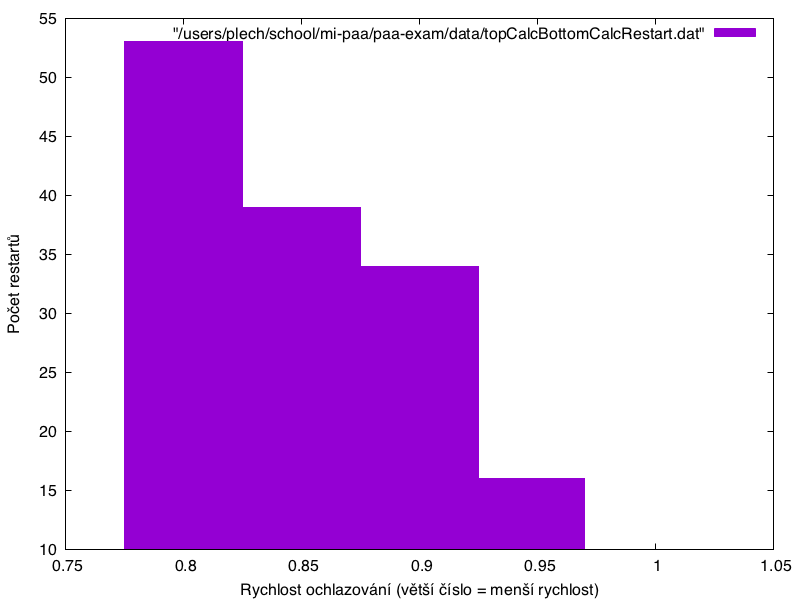
\includegraphics[width=\textwidth]{topCalcBottomCalcRestart}
\caption{Vývoj počtu restartů (průměr pro 100 běhů)}
\label{topCalcBottomCalcRestart}
\end{figure}

\begin{figure}[H]
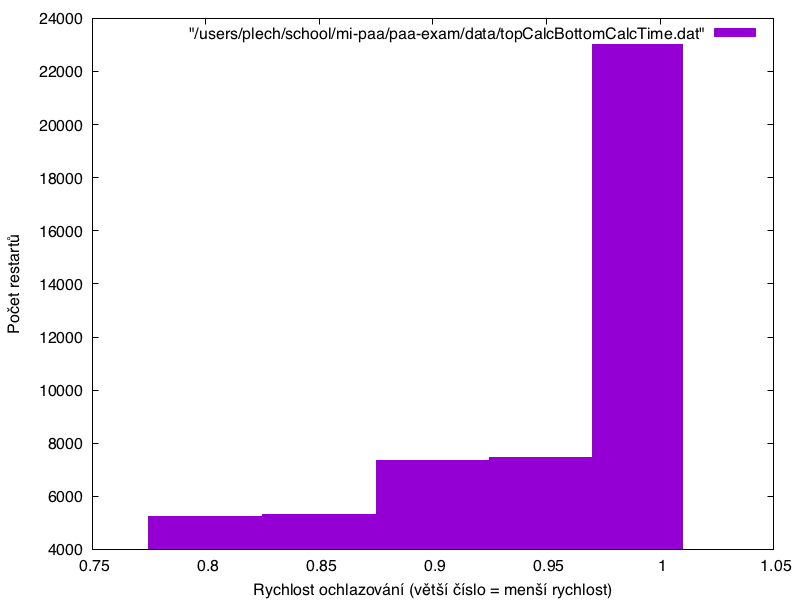
\includegraphics[width=\textwidth]{topCalcBottomCalcTime}
\caption{Vývoj doby trvání (průměr pro 100 běhů)}
\label{topCalcBottomCalcTime}
\end{figure}










\section{Závěr}

Je několik způsobů, jak implementovat metodu simulovaného ochlazování pro řešení problému vážené splnitelnosti booleovských formulí. V první řadě záleží na volbě, jak zacházet se skoky na stavy, které nejsou řešením, protože nemají všechny klauzule splněné. Zde jsem dospěl k názoru, že je třeba taková řešení penalizovat, a to tak, že do optimalizované hodnoty asymptoticky výrazně důležitěji započítáme počet splněných klauzulí než celkovou váhu. 

Dále záleží na volbě počáteční i koncové teploty. Zde jsem se rozhodl pro co nejobecnější přístup přes dynamický výpočet obojího.

Rychlost ochlazování je vhodná volit spíše rychlejší, protože ačkoli počet restartů s pomalejší rychlostí klesá, celkový čas výpočtu roste.

Všiml jsem si jedné zajímavé vlastnosti. Mnoho chodů algoritmu nenajde žádný přijatelný stav (dříve uvázne v lokálním minimu). Nicméně najde-li algoritmus nějaký platný výsledek, ve většině případů ještě v rámci téhož průchodu nalezne další, lepší výsledky (s větší vahou). Vypadá to, jako že v rámci lokálního minima, kde se nachází nějaké řešení, se mnohdy nachází řešení více.



\section*{Přílohy}

\begin{description}
    \item[sources.zip] Balík obsahující celý projekt v C++ spolu s CMakeLists.txt souborem pro CMake. V podsložce data se nacházejí tři zkušební instance v cnf formátu a různé výstupy a obrázky, z nichž ty podstatné jsou použity v tomto dokumentu.
\end{description}



\end{document}